\documentclass[final, hyperref, table]{beamer}
\mode<presentation>
{ 
\usetheme{TF}
 }

 \usepackage[english,francais]{babel} % "babel.sty"
% \usepackage{french}                  % "french.sty"
%  \usepackage{franglais}               % "franglais.sty" (a defaut)
  \usepackage{times}			% ajout times le 30 mai 2003
 
%% --------------------------------------------------------------
%% CODAGE DE POLICES ?
%% Si votre moteur Latex est francise, il est conseille
%% d'utiliser le codage de police T1 pour faciliter la césure,
%% si vous disposez de ces polices (DC/EC)
\usepackage[utf8]{inputenc}
\usepackage[T1]{fontenc}


%% ==============================================================
%\usepackage{graphicx}
\usepackage{amsmath,amsfonts}
%\usepackage[table]{xcolor}
\usepackage{subfigure}
\usepackage{fancybox}
%\usepackage{hyperref}
\usepackage{multicol}
\usepackage{wrapfig}
\usepackage{listings}
\usepackage{xcolor}
\usepackage[orientation=portrait,size=a0,scale=1.4]{beamerposter}

% Display a grid to help align images
%\beamertemplategridbackground[1cm]

%We will get the normal bibliography style (number or text instead of icon) by including the following code
\setbeamertemplate{bibliography item}[text]
\setbeamerfont{caption}{size=\footnotesize}
% listings settings
\definecolor{lstComments}{rgb}{1,0.2,0.2}
\definecolor{lstBkgrd}{rgb}{0.95,0.95,1}
\lstset{%
  language=Python, % the language of the code
  frame=single,  % adds a frame around the code
  commentstyle=\color{lstComments},% comment style
  backgroundcolor=\color{lstBkgrd},   % choose the background color
  basicstyle=\ttfamily\scriptsize,       % the size of the fonts that are used for the code
  keywordstyle=\color{blue},      % keyword style
  showstringspaces=false,          % underline spaces within strings only
}


\title[TELEMETA, an open web audio platform for ethnomusicological sound archives management]{An open web audio platform for ethnomusicological sound archives management and automatic analysis}

\author[Fillon, Pellerin, Brossier, Simonnot]{Thomas Fillon \inst{1,2}, Guillaume Pellerin\inst{1}, Paul Brossier\inst{1}, Jos{\'e}phine Simonnot\inst{3}}


\institute[Parisson]{\small
  \inst{1}%
  Parisson, France\\
  \inst{2}%
  LAM, Institut Jean Le Rond d'Alembert, UPMC Univ. Paris 06, UMR CNRS 7190,
    11 rue de Lourmel, 75015 Paris, France\\
 \inst{3}%
  CREM, LESC, UMR CNRS 7186, MAE, Université Paris Ouest Nanterre La Défense,
21 Allée de l'Université - 92023 Nanterre, France\\
%Thanks
\vskip1ex
 {\small \textcolor{red}{\emph{This work was partially done inside the DIADEMS project\\ funded by the French National Research Agency ANR (CONTINT)}}}
}

\date[13/06/2014]{13 june 2014}

\begin{document}

\begin{frame}[containsverbatim]{}
% ==================================
% --------- Résumé -----------------
% ==================================
  \begin{block}{Introduction}\small
    \begin{columns}
      \begin{column}{0.72\linewidth}
        \begin{itemize}
        \item Since 2007, ethnomusicologists from the \emph{Center for Research in
            \alert{Ethnomusicology}} (CREM) and engineers from Parisson have joint
          their effort to develop \emph{Telemeta}, a scalable and
          collaborative\alert{ \emph{open-source} web platform} for
          management of and access to \alert{digital sound archives}.
        \item A fully operational deployment of this platform is online since 2011 :
          \textbf{\og Sound archives of the CNRS - Musée de l'Homme\fg}: 
          \colorbox{yellow!50}
          {\normalsize \hskip1ex \textbf{\url{http://archives.crem-cnrs.fr} \hskip1ex }}
        \item The design of Telemeta focuses on the enhanced and
          collaborative user-experience in accessing audio items and
          their associated \alert{metadata} and on the possibility
          for the expert user to further enrich those metadata.
        \item It fits the professional requirements from both
          \alert{sound archivists and researchers} in \alert{ethnomusicology}.
   
        \end{itemize}
      \end{column}
      \begin{column}{0.26\linewidth}
        \begin{center}
          \includegraphics[scale=0.9]{img/logo_telemeta_1-1.pdf}\\
          \colorbox{yellow!50}{\Large
            \textbf{\url{http://telemeta.org/}}} \vskip1ex
          \colorbox{yellow!50} { Contact :
            \href{mailto:guillaume@parisson.com}{\{guillaume,thomas\}@parisson.com}}
        \end{center}
      \end{column}
    \end{columns}
    \vskip1ex
    Telemeta architecture relies on \emph{TimeSide}, an open
    \alert{audio processing framework} written in Python which:
    \begin{itemize}
    \item Provides \alert{decoding, encoding and streaming}
      methods for various formats together with a smart
      embeddable \alert{HTML audio player}.
    \item Includes a set of audio analysis plugins and
      additionally wraps several \alert{audio features
        extraction} libraries to provide \alert{automatic
        annotation, segmentation and musicological analysis}
    \end{itemize}
    % \colorbox{red!20}{\textbf{KEYWORDS : Sound archives, Metadata, Ethnomusicology, Database, Audio labelling, Web platform}}
  \end{block}
 
% ==================================
% --------- Corps -----------------
% ==================================
  \begin{columns}[T]
    \footnotesize
    % ==================================
    % --------- Colonne gauche ---------
    % ==================================
    \begin{column}[T]{.49\linewidth}
      % \begin{block}{Introduction}
      %   \vspace{-0.5cm}
      %   \textbf{Needs}\\
      %   \begin{itemize}
      %   \item In social sciences like anthropology and linguistics,
      %     researchers have to work on multiple types of multimedia
      %     documents such as photos, videos, sound recordings or
      %     databases.
      %   \item The need to easily access, visualize and annotate
      %     such materials can be problematic given their diverse formats,
      %     sources and given their chronological nature.
      %   \end{itemize}
        
 
      %   \vspace{-0.5cm}
      % \end{block}

      \begin{block}{Web audio content management features and architecture}
        \vspace{-0.5cm}  
        \begin{itemize}
        \item \emph{Telemeta} is a free and open source ({\scriptsize CeCILL
            Free Software License Agreement}) web audio content management
          system which introduces efficient and secure methods for
          \alert{backuping}, \alert{indexing}, \alert{transcoding}, \alert{analysing} and \alert{publishing} any
          digitalized audio file with its metadata.
        \item \emph{Telemeta} is ideal for
          professional collaborators who wants to easily organize, backup, archive and
          publish documented sound collections of audio files, CDs,
          digitalized vinyls and magnetic tapes over a strong database in
          accordance with \alert{open web standards}.
        \item \emph{Telemeta} architecture
          is \alert{flexible} and can easily be adapted to particular database
          organization of a given sound archives.
        \end{itemize}
        
        The main features of \emph{Telemeta} are:
        \vspace{-0.1cm}
        \begin{itemize}
        \item \alert{Pure HTML} web user interface including high level \alert{search engine}
        \item \alert{Smart workflow management} with contextual user lists, profiles and rights
        \item Model-View-Controller (\alert{MVC}) architecture 
        \item Strong Structured Query Language (\alert{SQL}) or Oracle backend
        \end{itemize}
        Beside database management, the audio support is mainly provided through an external component, \emph{TimeSide}.
        
      \end{block}
      \begin{block}{Metadata}
        \vspace{-0.5cm}
        \begin{itemize}
        \item In addition to the audio data, an efficient and \alert{dynamic
            management} of the associated metadata is also required.
        \item Dynamically handling metadata in a \alert{collaborative} manner optimises
          the continuous process of knowledge gathering and enrichment of
          the materials in the database.
        \item Interoperability : integration of the metadata standards protocols \alert{Dublin Core}
          and \alert{OAI-PMH} (Open Archives Initiative Protocol for Metadata
          Harvesting) \cite{DublinCore,OAI-PMH}.
        \end{itemize}
        
        \textbf{Contextual Information}\\
        In ethnomusicology, contextual information could be geographic, cultural and musical. It could also store archive related information and include related materials in any multimedia format. 
        
        \textbf{Annotations and segmentation}\\
        Metadata also consist in temporal information such as:
        \begin{itemize}
        \item a list of \alert{time-coded markers} associated with annotations
        \item a list of of \alert{time-segments} associated with labels (\emph{in development}) .
        \end{itemize}
        The ontology for those labels is relevant for ethnomusicology (e.g. speech versus singing voice segment, chorus, ...).
        It should be noted that annotations and segmentation can be done either by a human expert or by some automatic signal processing analysis.
      \end{block}
      
      \begin{block}{Sound archives of the CNRS - Musée de l'Homme}
        The ressources are available to researchers and to the extent possible, the public, in compliance with the intellectual and moral rights of musicians and collectors.
        %\begin{columns}[T]
         % \begin{column}{0.27\linewidth}
            Theses archives are the most important in Europe:
            \begin{itemize}
            \item Nearly 3,500 hours of recordings of unpublished field.
            \item Approximately 3700 hours of material published (more than
              5000 discs, many of which are very rare).
            \end{itemize}
            
            The platform allows researchers to publish the ressources they have collected together with they research work. It also allows to exchange data online with other researchers or communities producing their music in their home countries through collaborative tools like markers and comments.
            
Telemeta is also used as a support for teachers in anthropology or ethnomusicology as it provides the students an access to ressources for lessons, academic works and exams.
            
          %\end{column}
          %\begin{column}{0.7\linewidth}
            %\centering
            \begin{center}
              \fbox{\includegraphics[width=0.8\linewidth]{../img/telemeta_screenshot_en_2.png}}
            \end{center}

          %\end{column}
        %\end{columns}

      \end{block}
      
      
    \end{column}
% ==================================
% ------- Colonne droite -----------
% ==================================
\section{TimeSide}
\begin{column}[T]{.49\linewidth}
\subsection{TimeSide architecture}
  \begin{block}{TimeSide : open web audio processing framework}
One specificity of the \emph{Telemeta} architecture is to rely on an external component, \emph{TimeSide}, that offers audio player integration together with low and high level audio signal processing capabilities.

\begin{center}
  \colorbox{yellow!50}{\bf \hskip3ex \url{https://github.com/yomguy/TimeSide/} \hskip3ex  }
\end{center}
\begin{columns}[T]
  %\begin{minipage}{0.34\linewidth}
  \begin{column}{.36\linewidth}
    \begin{beamerboxesrounded}[shadow=true]{Functionality}
       \begin{itemize}
       \item \alert{Do} asynchronous and fast audio processing with
         Python.
       \item \alert{Decode} ANY audio or video format into numpy arrays
         thanks to Gstreamer.
       \item \alert{Analyze} audio content with some external audio
         feature extraction libraries.
       \item \alert{Organize}, \alert{serialize} and \alert{save}
         analysis metadata through various formats.
       \item \alert{Draw} various waveforms, spectrograms and
        other representations from audio analysis.
      \item \alert{Transcode} audio data in various media formats and
        stream them through web apps.
      \item \alert{Playback}, \alert{index}, \alert{tag} and
        \alert{interact} on demand with a smart high-level HTML5
        extensible player.
      \end{itemize}
    \end{beamerboxesrounded}

  \end{column}

  %\end{minipage}
  %\begin{minipage}{0.65\linewidth}
  \begin{column}[T]{0.6\linewidth}
    \begin{beamerboxesrounded}[shadow=true]{TimeSide Architecture}
       \centering
        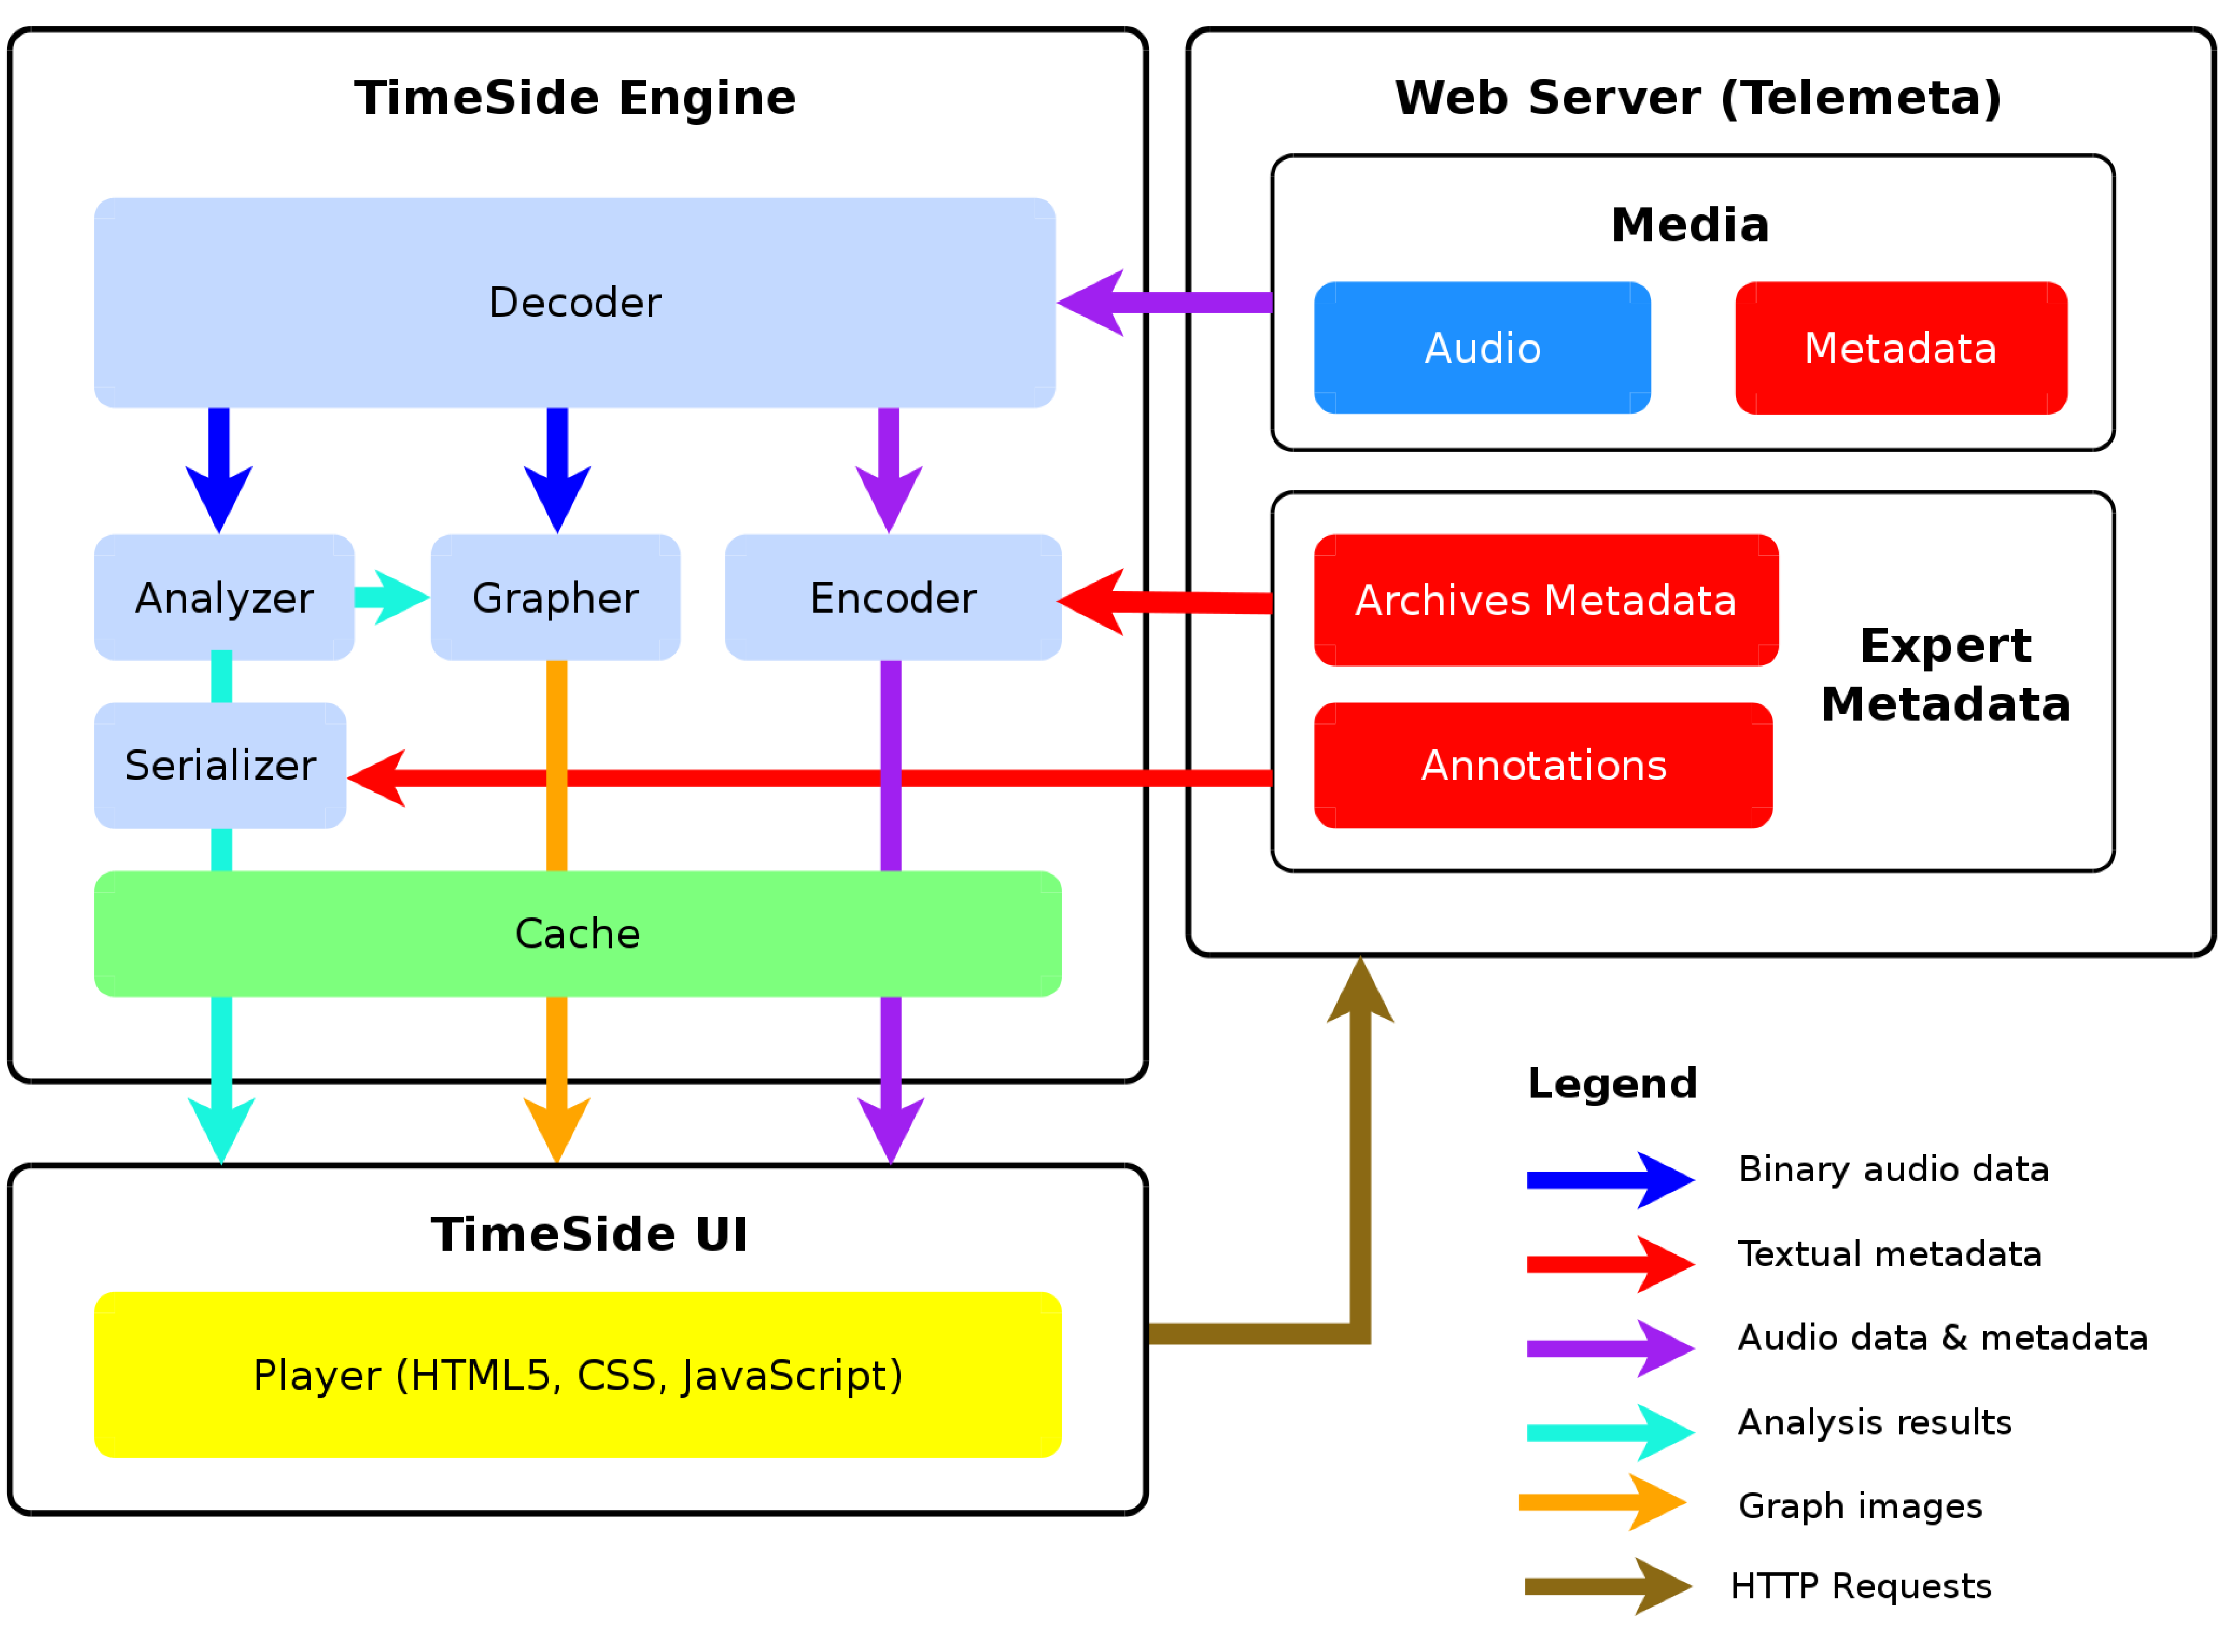
\includegraphics[width=\linewidth]{../img/timeside_schema_v3.pdf}
      \end{beamerboxesrounded}

  \end{column}

  %\end{minipage}
\end{columns}

\begin{beamerboxesrounded}%
       [shadow=true]%
       {Audio features extraction}
  TimeSide incorporates some state-of-the-art audio feature extraction
  libraries such as:

  \begin{itemize}
  \item \textbf{Aubio: \colorbox{yellow!50}{\hskip1ex
        \url{http://aubio.org} \hskip1ex }} \cite{brossierPhD}
  \item \textbf{Yaafe: \colorbox{yellow!50}{\hskip1ex
        \url{http://yaafe.sourceforge.net}\hskip1ex }}
    \cite{yaafe_ISMIR2010}
  \item \textbf{Vamp plugins: \colorbox{yellow!50}{\hskip1ex
        \url{http://www.vamp-plugins.org}\hskip1ex }}
    \cite{vamp-plugins}
  \end{itemize}

  Given the extracted features, every sound item in a given collection
  can be automatically analyze. The results of this analysis can be
  displayed as a support to ethnomusicological studies. 
\end{beamerboxesrounded}

%\end{block}



%\begin{block}{TimeSide Architecture}


\end{block}

\begin{block}{Code Example (Python)}
\begin{columns}[T]
  \begin{column}[T]{0.6\linewidth}
    \lstinputlisting{code_example.py}
  \end{column}
 
  \begin{column}[T]{0.35\linewidth}
    \begin{beamerboxesrounded}[shadow=true]{Results}
      \begin{figure}
        \centering
        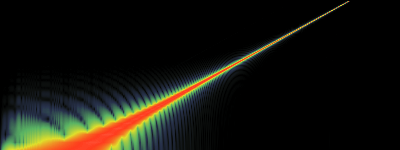
\includegraphics[width=\linewidth]{img/spectrogram.png}
        \caption{Spectrogram (sweep signal)}
      \end{figure}
        \vskip5ex
    \begin{lstlisting}
 Level Analyzer Max:[-6.021] 
 Level Analyzer RMS:[-9.856]
    \end{lstlisting}
\end{beamerboxesrounded}
  \end{column}
\end{columns}
  \end{block}

  \begin{block}{Ongoing developments}
\vspace{-1cm}
    \begin{multicols}{2}[]
      The main goal is to turn Telemeta into a fully operational platform with a modern web interface for:
        \begin{itemize}
        \item \alert{Annotate} multimedia items by time segments supporting both free annotations and ontology-based annotations
        \item Efficiently \alert{visualize} results from analysis from various data types together with X-Y zoom capability and audio synchronization
        
        \item Provide TimeSide with a RESTful web API to design, manage and run
          analysis on large audio corpus and serialize results
        \item Increase the analysis functionality with various automatic analysis and annotation tools for speech, audio, Music Information Retrieval and ethnomusicology (DIADEMS project).
\end{itemize}
\end{multicols}
\end{block}

\begin{block}{Références}\tiny
\bibliographystyle{plain}
%\label{sec:ref}
\vspace{-1cm}
\begin{multicols}{2}[]
\bibliography{../fma2014_Telemeta}
\end{multicols}
\end{block}
  
\end{column}
\end{columns}
\end{frame}
\end{document}